\problemname{Family Fares}

\tikzstyle{vertex}=[auto=left,circle,fill=black!25,minimum size=20pt,inner sep=0pt]

After a long time apart, your family will gather next year for a reunion in an idyllic village in
the centre of the country. Since everybody lives apart, most will need to travel by train.

You are in charge of finding the best deal on tickets. Everyone must take an optimal route,
that is to say they may only travel a route if no other route is shorter.

Two types of ticket are available: \emph{individual} or \emph{group}. All tickets come with a start
and destination between which to travel. Individual tickets are unlimited and the price is equal to the
shortest distance in kilometres between stations.

Group tickets are more complicated. First, you may only buy at most one and it must be for a set list
of people. There is no limit to the number of people named, but all must be present. The ticket is
priced according to the number of named persons.

\begin{figure}[!h]
\centering
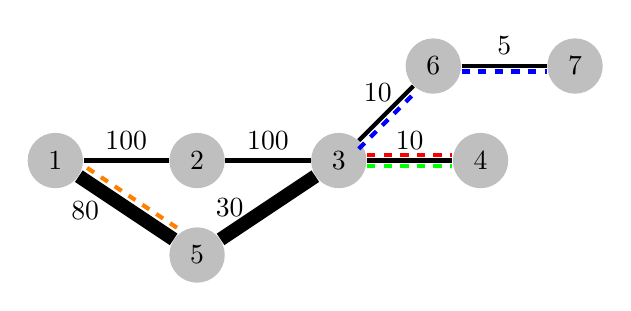
\begin{tikzpicture}[scale=0.6]
    \node[vertex] (n1) at (0,0) {$1$};
    \node[vertex] (n2) at (3,0) {$2$};
    \node[vertex] (n3) at (6,0) {$3$};
    \node[vertex] (n4) at (9,0) {$4$};
    \node[vertex] (n5) at (3,-2) {$5$};
    \node[vertex] (n6) at (8,2) {$6$};
    \node[vertex] (n7) at (11,2) {$7$};
  
    \draw[line width=1.5pt] (n1) -- (n2) node [midway,above] {$100$};
    \draw[line width=1.5pt] (n2) -- (n3) node [midway,above] {$100$};
    \draw[red,dashed,line width=1.5pt,transform canvas={yshift=2pt}] (n3) -- (n4) node [midway,above] {};
    \draw[line width=1.5pt,dashed,green,transform canvas={yshift=-2pt}] (n3) -- (n4) node [midway,above] {};
    \draw[line width=1.5pt,dashed,blue,transform canvas={yshift=-3pt}] (n3) -- (n6) node [midway,above] {};
    \draw[line width=1.5pt] (n3) -- (n4) node [midway,above] {$10$};
    \draw[line width=1.5pt](n3) -- (n6) node[xshift=-3pt] [midway,above] {$10$};
    \draw[line width=1.5pt](n6) -- (n7) node [midway,above] {$5$};
    \draw[line width=1.5pt,dashed,blue,transform canvas={yshift=-2pt}] (n6) -- (n7) node [midway,above] {};
    \draw[line width=5pt](n1) -- (n5) node[xshift=-4pt,yshift=-1pt] [midway,left] {$80$};
    \draw[line width=1.5pt,dashed,orange,transform canvas={yshift=3pt,xshift=3pt}] (n1) -- (n5) node [midway,above] {};
    \draw[line width=5pt](n5) -- (n3) node[xshift=-3pt] [midway,left] {$30$};
    
\end{tikzpicture}
\caption{Sample 2. Group or individual tickets are shown by thick or thin lines, respectively.}
\end{figure}

\vspace{-0.5cm}
\section*{Input}
	\begin{itemize}
		\item One line with four integers: $n$ ($2 \le n \le 1000$), the number of stations, $m$
			($n-1 \le m \le 10^5$), the number of connections between stations, $p$ ($1 \le p \le 100$),
			the number of family members, and $g$ ($1 \le g \le 10^6$), the cost per person of a group ticket.
		\item One line with $p$ integers $v_i$ ($1 \le v \le n$), meaning that family member $i$ starts at station $v_i$.
		\item $m$ further lines, each with three integers $a$, $b$, and $c$ (${1 \le a,b \le n}$, $a\neq b$, and ${1 \le c \le 10^6}$),
			indicating that there is a bidirectional connection between stations $a$ and $b$ with a length of $c$ kilometres.
	\end{itemize}
  Each pair of distinct stations has at most one direct connection and every station can be reached from any other station.
  Station number $1$ serves the idyllic village.

\section*{Output}
	Output the total amount you must spend so that every family member can travel from their starting station to the idyllic village.
